\begin{figure}
    \begin{center}
    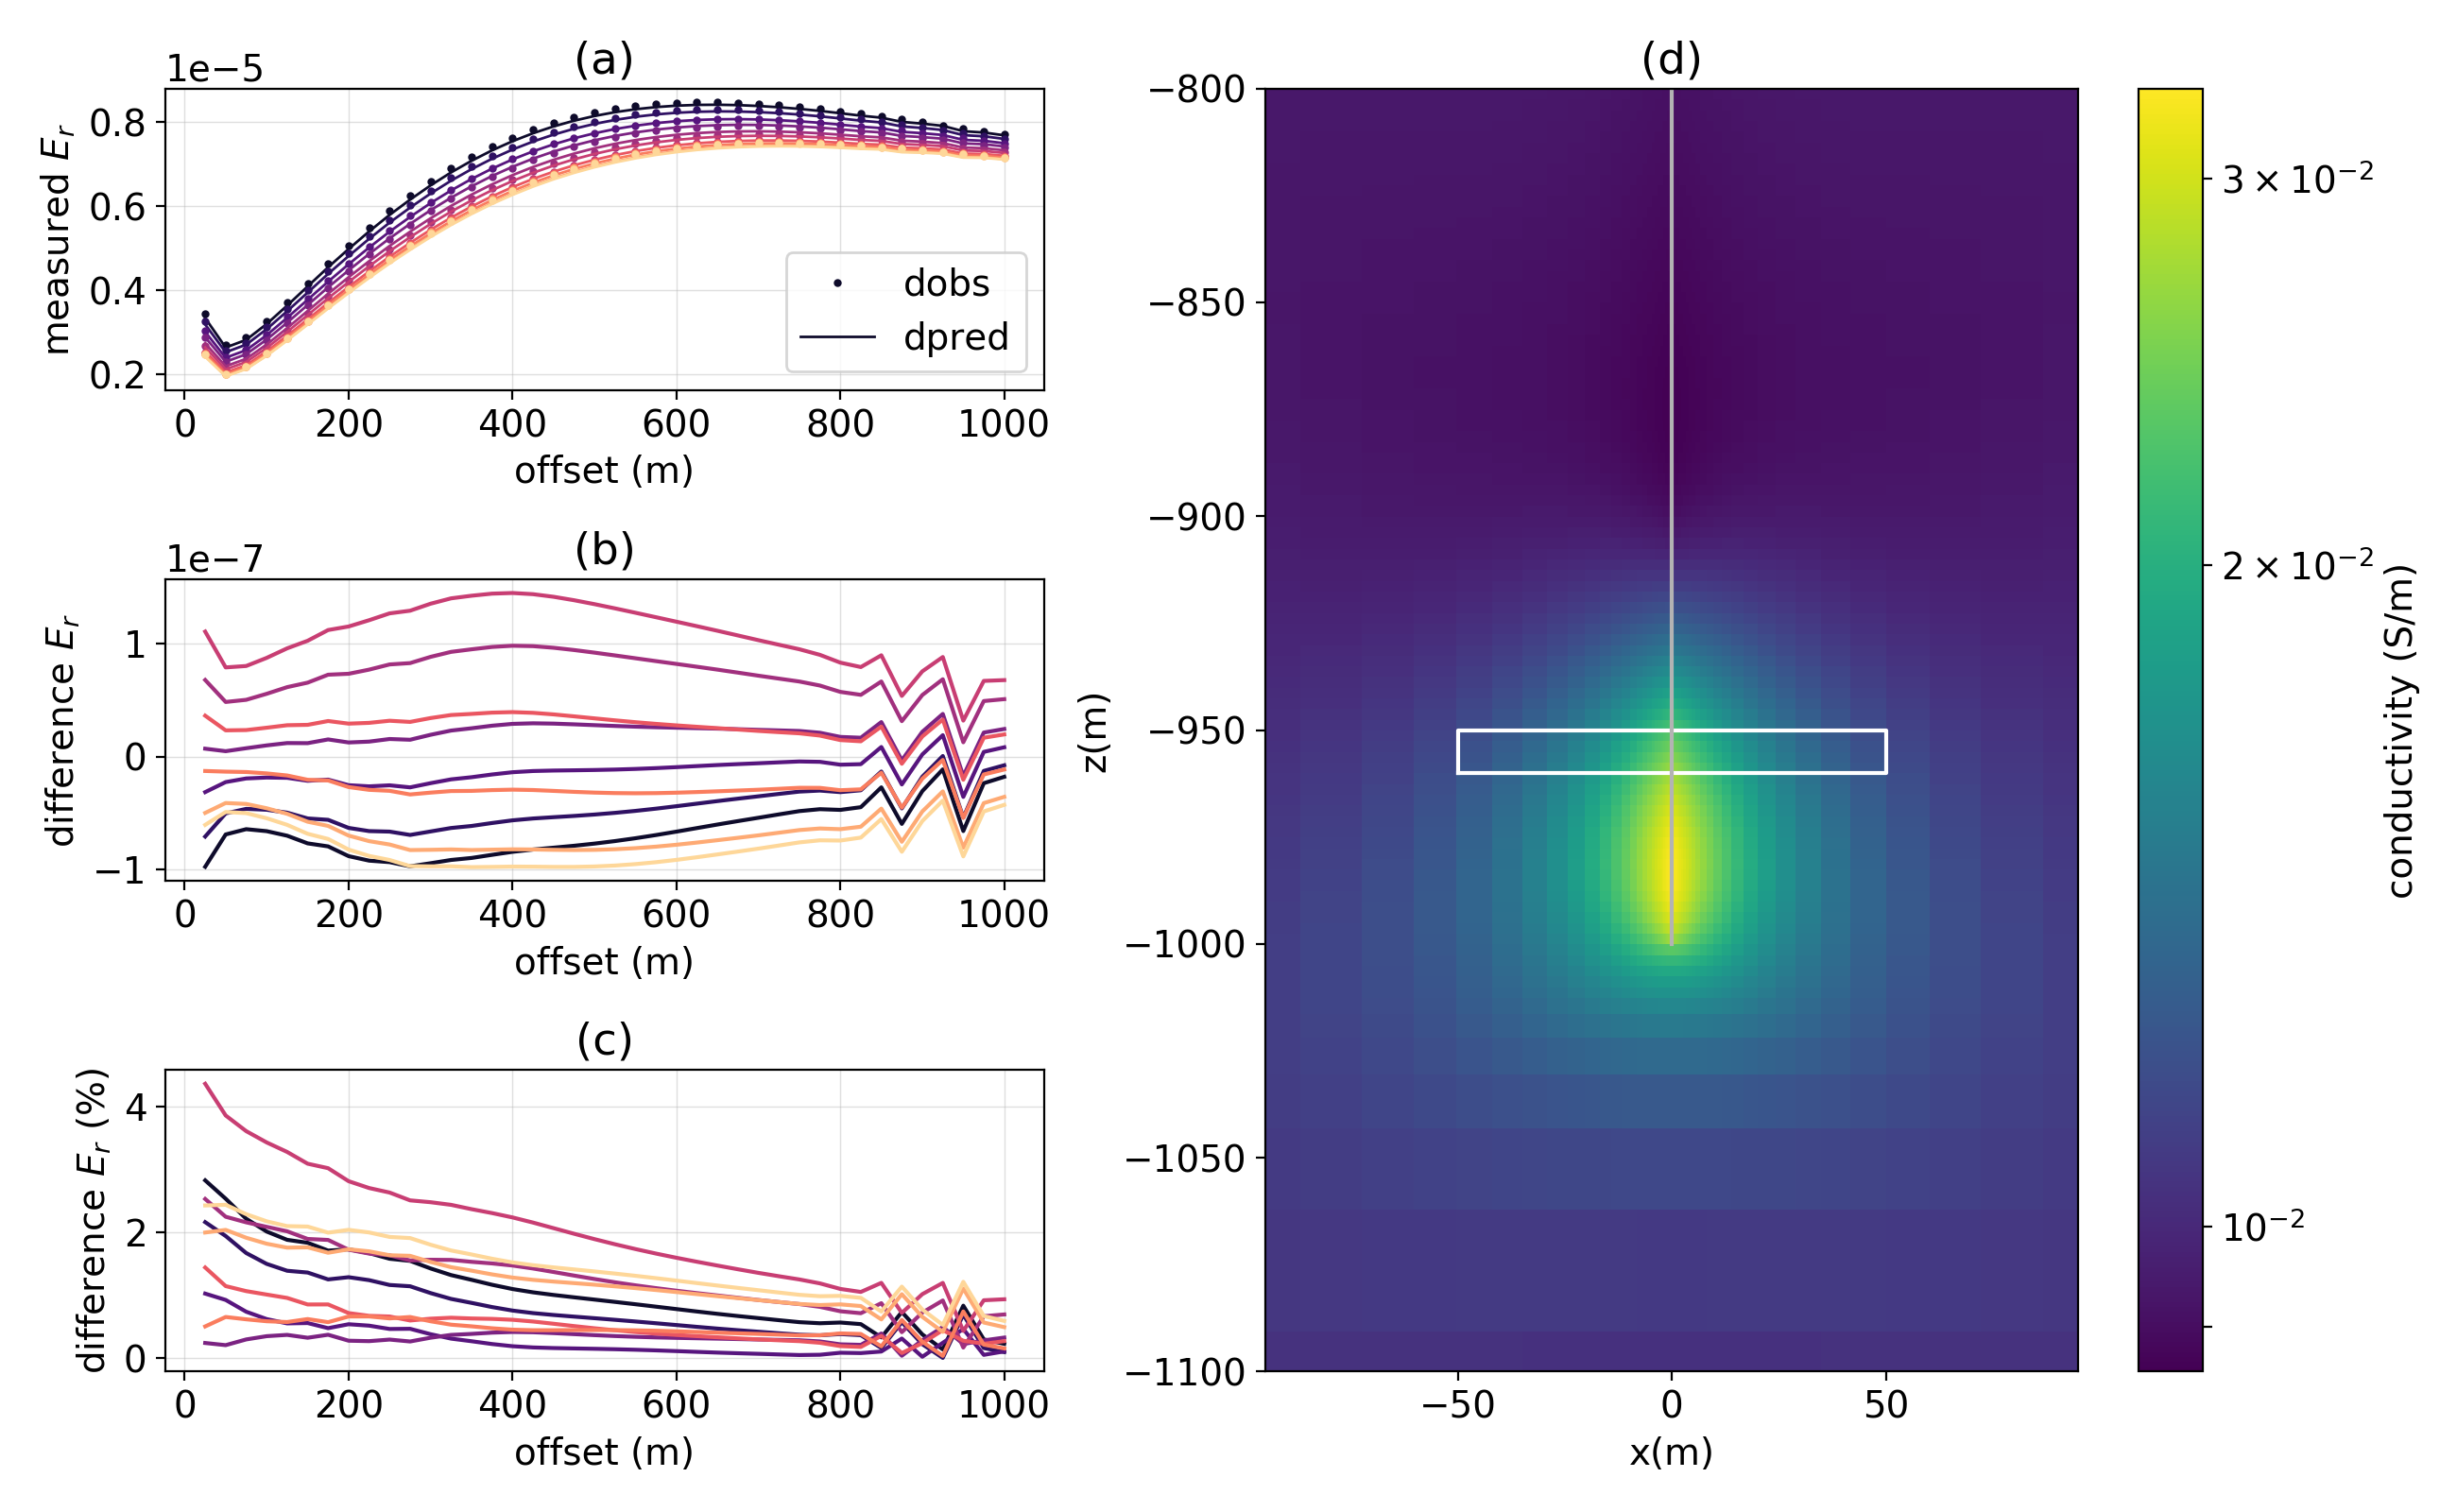
\includegraphics[width=0.8\textwidth]{figures/inversion/dc_smooth_inversion_1e-01.png}
    \end{center}
\caption{
    (a) Observed and predicted radial electric field data,
    (b) difference between the observed and predicted data (V/m),
    (c) difference between the observed and predicted data as a percentage of the observed data,
    and (d) conductivity model recovered in the inversion.
    The colors in (a), (b), and (c) indicate the source location as shown in Figure \ref{fig:dc_casing_initial_data}.
    The white outline in (d) outlines the true geometry of the fracture zone and the grey line shows the location of the wellbore.
    The data are fit to a global $\chi$-factor $<$ 0.1 and the inversion took 3 iterations.
}
\label{fig:dc_smooth_inversion_1e-01}
\end{figure}
